\section{Musterlösung Bootprozess}

\subsection{Printk während des Booten}

Der Bootprozess, welcher in der Vorlesung besprochen wurde, soll nun experimentel überprüft werden.
Dabei sollen mit Hilfe von \emph{printk()} Einträge ins Kernellog gemacht werden. \\

Erstellen Sie zunächst einen neuen Ordner \emph{boot} unter \emph{workspace}

\begin{figure}[h!]
   \begin{center}
      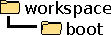
\includegraphics{images/boot_dirs}
   \end{center}
   \caption{Ordnerstruktur für die Aufgabe 2}
\end{figure}

Entpacken Sie mit den folgenden Befehlen den Linux-Kernel.

\begin{lstlisting}
$ cd ~/workspace/boot
$ cp /usr/src/linux-source-*.tar.bz2 .
$ tar xjf linux-source-*.tar.bz2
\end{lstlisting}

Modifizieren Sie nun die Funktion \emph{start\_kernel()} wie in Listing \ref{boot_start_kernel2} zu sehen ist,
indem Sie die \emph{printk()}-Statements hinzufügen.

\begin{lstlisting}[label=boot_start_kernel2,caption=init/main.c]
// [..]

asmlinkage void __init start_kernel(void)
{
        char * command_line;
        extern const struct kernel_param __start___param[], __stop___param[];

        /* modified tux */
        printk(KERN_INFO "#### tux: start_kernel() ####");

        smp_setup_processor_id();

       // [..]
\end{lstlisting}

Dasselbe machen Sie mit der \emph{rest\_init()}...

\begin{lstlisting}[label=boot_rest_init,caption=init/main.c]
static noinline void __init_refok rest_init(void)
{
        int pid;

        /* modified by tux */
        printk(KERN_INFO "#### tux: rest_init() ####");

        /* [..] */

        /* modified by tux */
        printk(KERN_INFO "#### tux: before cpu_idle()) ####");

        /* Call into cpu_idle with preempt disabled */
        preempt_disable();
        cpu_idle();

        /* modified by tux */
        printk(KERN_INFO "#### tux: after cpu_idle()) ####");
}
\end{lstlisting}

und der \emph{kernel\_init()}-Funktion.

\begin{lstlisting}[label=boot_kernel_init,caption=init/main.c]
static int __init kernel_init(void * unused)
{
        /* modified by tux */
        printk(KERN_INFO "#### tux: kernel_init() ####");

        /*
         * Wait until kthreadd is all set-up.
         */
        wait_for_completion(&kthreadd_done);

        /* [..] */

        init_post();

        /* modified by tux */
        printk(KERN_INFO "#### tux: after kernel_init() ####");

        return 0;
}
\end{lstlisting}

Anschliessend kompilieren Sie den Kernel. Achten Sie auf Kompilierungsfehler und beheben
Sie diese bei Bedarf.
\begin{lstlisting}
$ cd ~/workspace/boot/linux-source-*
$ make
\end{lstlisting}

Danach installiern Sie den Kernel mit folgendem Befehl:
\begin{lstlisting}
$ make modules_install install
\end{lstlisting}

Starten Sie die virtuelle Maschine neu und wählen Sie im Grub-Menü (Abbildung \ref{boot_grub2}) den neuen Kernel aus.
\begin{figure}[h!]
   \begin{center}
      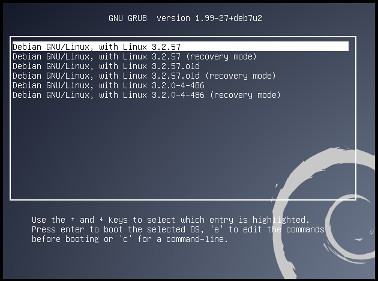
\includegraphics{images/boot_grub}
   \end{center}
   \caption{Auswahl im Grub-Menu}
   \label{boot_grub2}
\end{figure}

Analysieren Sie nach dem Boot das Kernellog mit \emph{dmesg}.

\begin{lstlisting}
$ dmesg | less
\end{lstlisting}

Was stellen Sie dabei fest? \\

\underline{\textcolor{red}{Es werden nur 4 von 5 printk() Ausgaben angezeigt.}\hspace{0.5\textwidth}} \\

Kopieren Sie die Ausgabe des folgenden Befehls in die folgenden Zeilen.
\begin{lstlisting}
$ dmesg | grep "#### tux"
\end{lstlisting}

[00000.000000] \underline{\smash{\textcolor{red}{\#\#\#\# tux: start\_kernel() \#\#\#\#\hspace{0.2\textwidth}}}} \newline
[00000.000000] \underline{\smash{\textcolor{red}{\#\#\#\# tux: rest\_init() \#\#\#\#\hspace{0.24\textwidth}}}} \newline
[00000.000000] \underline{\smash{\textcolor{red}{\#\#\#\# tux: kernel\_init() \#\#\#\#\hspace{0.21\textwidth}}}} \newline
[00000.000000] \underline{\smash{\textcolor{red}{\#\#\#\# tux: before cpu\_idle() \#\#\#\#\hspace{0.16\textwidth}}}} \newline
[00000.000000] \underline{\hspace{0.5\textwidth}} \newline
[00000.000000] \underline{\hspace{0.5\textwidth}} \newline
[00000.000000] \underline{\hspace{0.5\textwidth}} \newline

\subsection{Init-Programm}

Im nächsten Schritt wollen wir das Init-Programm auswechseln. Hierzu müssen wir die 
Bootparameter von Linux anpassen. Die Bootparameter müssen im Bootloader konfiguriert 
werden. Editieren Sie hierfür mit Root-Rechten
die Datei \emph{/boot/grub/grub.cfg}. \\

Gehen Sie wie folgt vor:
\begin{itemize}
   \item Suchen Sie in der Datei nach \emph{menuentry}.
   \item Kopieren Sie den gesammten ersten Menuentry.
   \item Ändern Sie den Namen zu \emph{Boot to bash}.
   \item Fügen Sie den Bootparameter \emph{init=/bin/bash} hinzu.
\end{itemize}

Der neue Eintrag sollte ähnlich des Listing \ref{boot_grubmenu2} aussehen.

\begin{lstlisting}[label=boot_grubmenu2,caption=/boot/grub/grub.cfg]
menuentry 'Boot to bash' --class debian --class gnu-linux --class gnu --class os {
        load_video
        insmod gzio
        insmod part_msdos
        insmod ext2
        set root='(/dev/sda,msdos1)'
        search --no-floppy --fs-uuid --set=root a2a446aa-571f-4041-b6ce-d5f62f336ba5
        echo    'Loading Linux 3.2.57 ...'
        linux   /boot/vmlinuz-3.2.57 root=UUID=a2a446aa-571f-4041-b6ce-d5f62f336ba5 ro  quiet init=/bin/bash
        echo    'Loading initial ramdisk ...'
        initrd  /boot/initrd.img-3.2.57
}
\end{lstlisting}

Speicheren Sie die Datei und starten Sie die virtuelle Maschine neu. Wählen Sie im Grub-Menu den
neuen Eintrag \emph{Boot to bash} aus.

\clearpage

Was ist passiert? \\

\underline{\textcolor{red}{Das System bootet direkt in die Bash-Shell}\hspace{0.5\textwidth}} \\


Was sehen Sie bei der Eingabe des Befehls von \emph{whoami}? \\

\underline{\textcolor{red}{Ausgabe: \emph{root}. Das Init-Programm wird immer als Root ausgeführt.}\hspace{0.23\textwidth}}
